\section{Lissajous-based exhibits}

Les figures Lissajous (que reben el nom del matemàtic francès Jules Antoine Lissajous) són corbes determinades per la intersecció de dos moviments oscil·lants perpendiculars. Matemàticament, les seves coordenades $x,y$ al pla són definides per cada instant de temps $t$ a les fórmules:
$$\left\{ \begin{array}{rcl}
x &=& \sin(a\cdot t) \\
y &=& \sin(b\cdot t + \varphi)
\end{array} \right. $$
on $t$ és el paràmetre del temps (angle), $a$ i $b$ són les dues freqüències, i $\varphi$ és el desfasament entre una i altra. Per diferents valors de temps $t$, les equacions formen una corba dins un quadrat. La seva forma exacta depèn bàsicament de la ràtio numèrica de les dues freqüències. Si $a=b$, o $a/b=1$, llavors la figura es tanca després d'un període i el resultat és una línia o una el·lipse. Si $a/b = 3/2$, la corba tanca després de $3\cdot 2=6$ cicles i és força neta. En general, ràtios de nombres petits resulten en corbes simples. Altrament, si els nombres	tenen ràtios més complexes, com ara $a/b = 23/22$, la corba es tanca després de molts cicles (concretament $22\cdot 23=506$ cicles) i la figura resultant és més densa i desordenada. Per això, les figures de Lissajous són una eina per visualitzar quan dos nombres tenen una ràtio simple.

En aquest cas, les nostres oscil·lacions són el so, i la freqüència del so es percep com el to. A la música, una idea fonamental que es remunta fins a Pitàgores, és que els sons amb freqüències amb ràtios més petites sonen consonants, i freqüències amb ràtios més complicades són menys consonants. Per aquest motiu les figures de Lissajous s'utilitzen per visualitzar consonància o dissonància. Els intervals consonants clàssics són l'octava (ràtio 2:1), la quinta (ràtio 3:2) i la tercera major (ràtio 5:4).

També és possible tenir corbes de Lissajous tridimensionals, anàlogues a les de dues dimensions, però amb tres vibracions perpendiculars en comptes de dues. Tres notes sonant alhora formant un acord de triada, que són la base per la composició musical. En afinació d'entonació justa, els acords majors els formen notes amb ràtios 4:5:6 i els acords menors notes amb ràtios 10:12:15.

És especialment remarcable que aquestes relacions ens produeixen sentiments d'``alegria'' amb els acords majors i ``tristesa'' amb els menors. Jugar amb aquestes relacions es transforma en una aventura per a la composició d'una peça que aconsegueixi transportar emocions.


\section{Galeria de Lissajous}
Les sis figures d'aquest apartat són representacions artístiques de figures de Lissajous. Per crear-les, l'artista Ryan Cashman va començar amb una corba a l'espai definida per dues ones sinusoidals. Això és una figura de Lissajous, però també està modulada per una segona oscil·lació. Amb la ràtio de freqüència escollida, la corba es mou al voltant de si mateixa passant molt a prop però no exactament sobre si mateixa. El programa calcula punts a intervals regulars durant la corba, creant vèrtexs. Els vèrtexs es connecten en ordre per crear la corba base de la forma. Després es dibuixen línies entre qualsevol parell de vèrtexs que estiguin prou a prop a l'espai per crear una representació de la superfície que recorda a una teranyina. Les freqüències escollides per cada imatge són acords en afinació de temperament igual.


Matemàticament, la posició $x$ (eix horitzontal) i la $y$ (eix vertical) de cada vèrtex es calcula amb la fórmula:
$$\left\{ \begin{array}{rcl}
x &=& \sin(f_X\cdot t + \varphi) \cdot \cos(m_X \cdot t) \\
y &=& \sin(f_Y\cdot t + \varphi) \cdot \cos(m_Y \cdot t)
\end{array} \right. $$
on també hi ha, de forma addicional, $m_X$ i $m_Y$ que en són els coeficients de modulació.

\begin{figure}[!h]
\centering
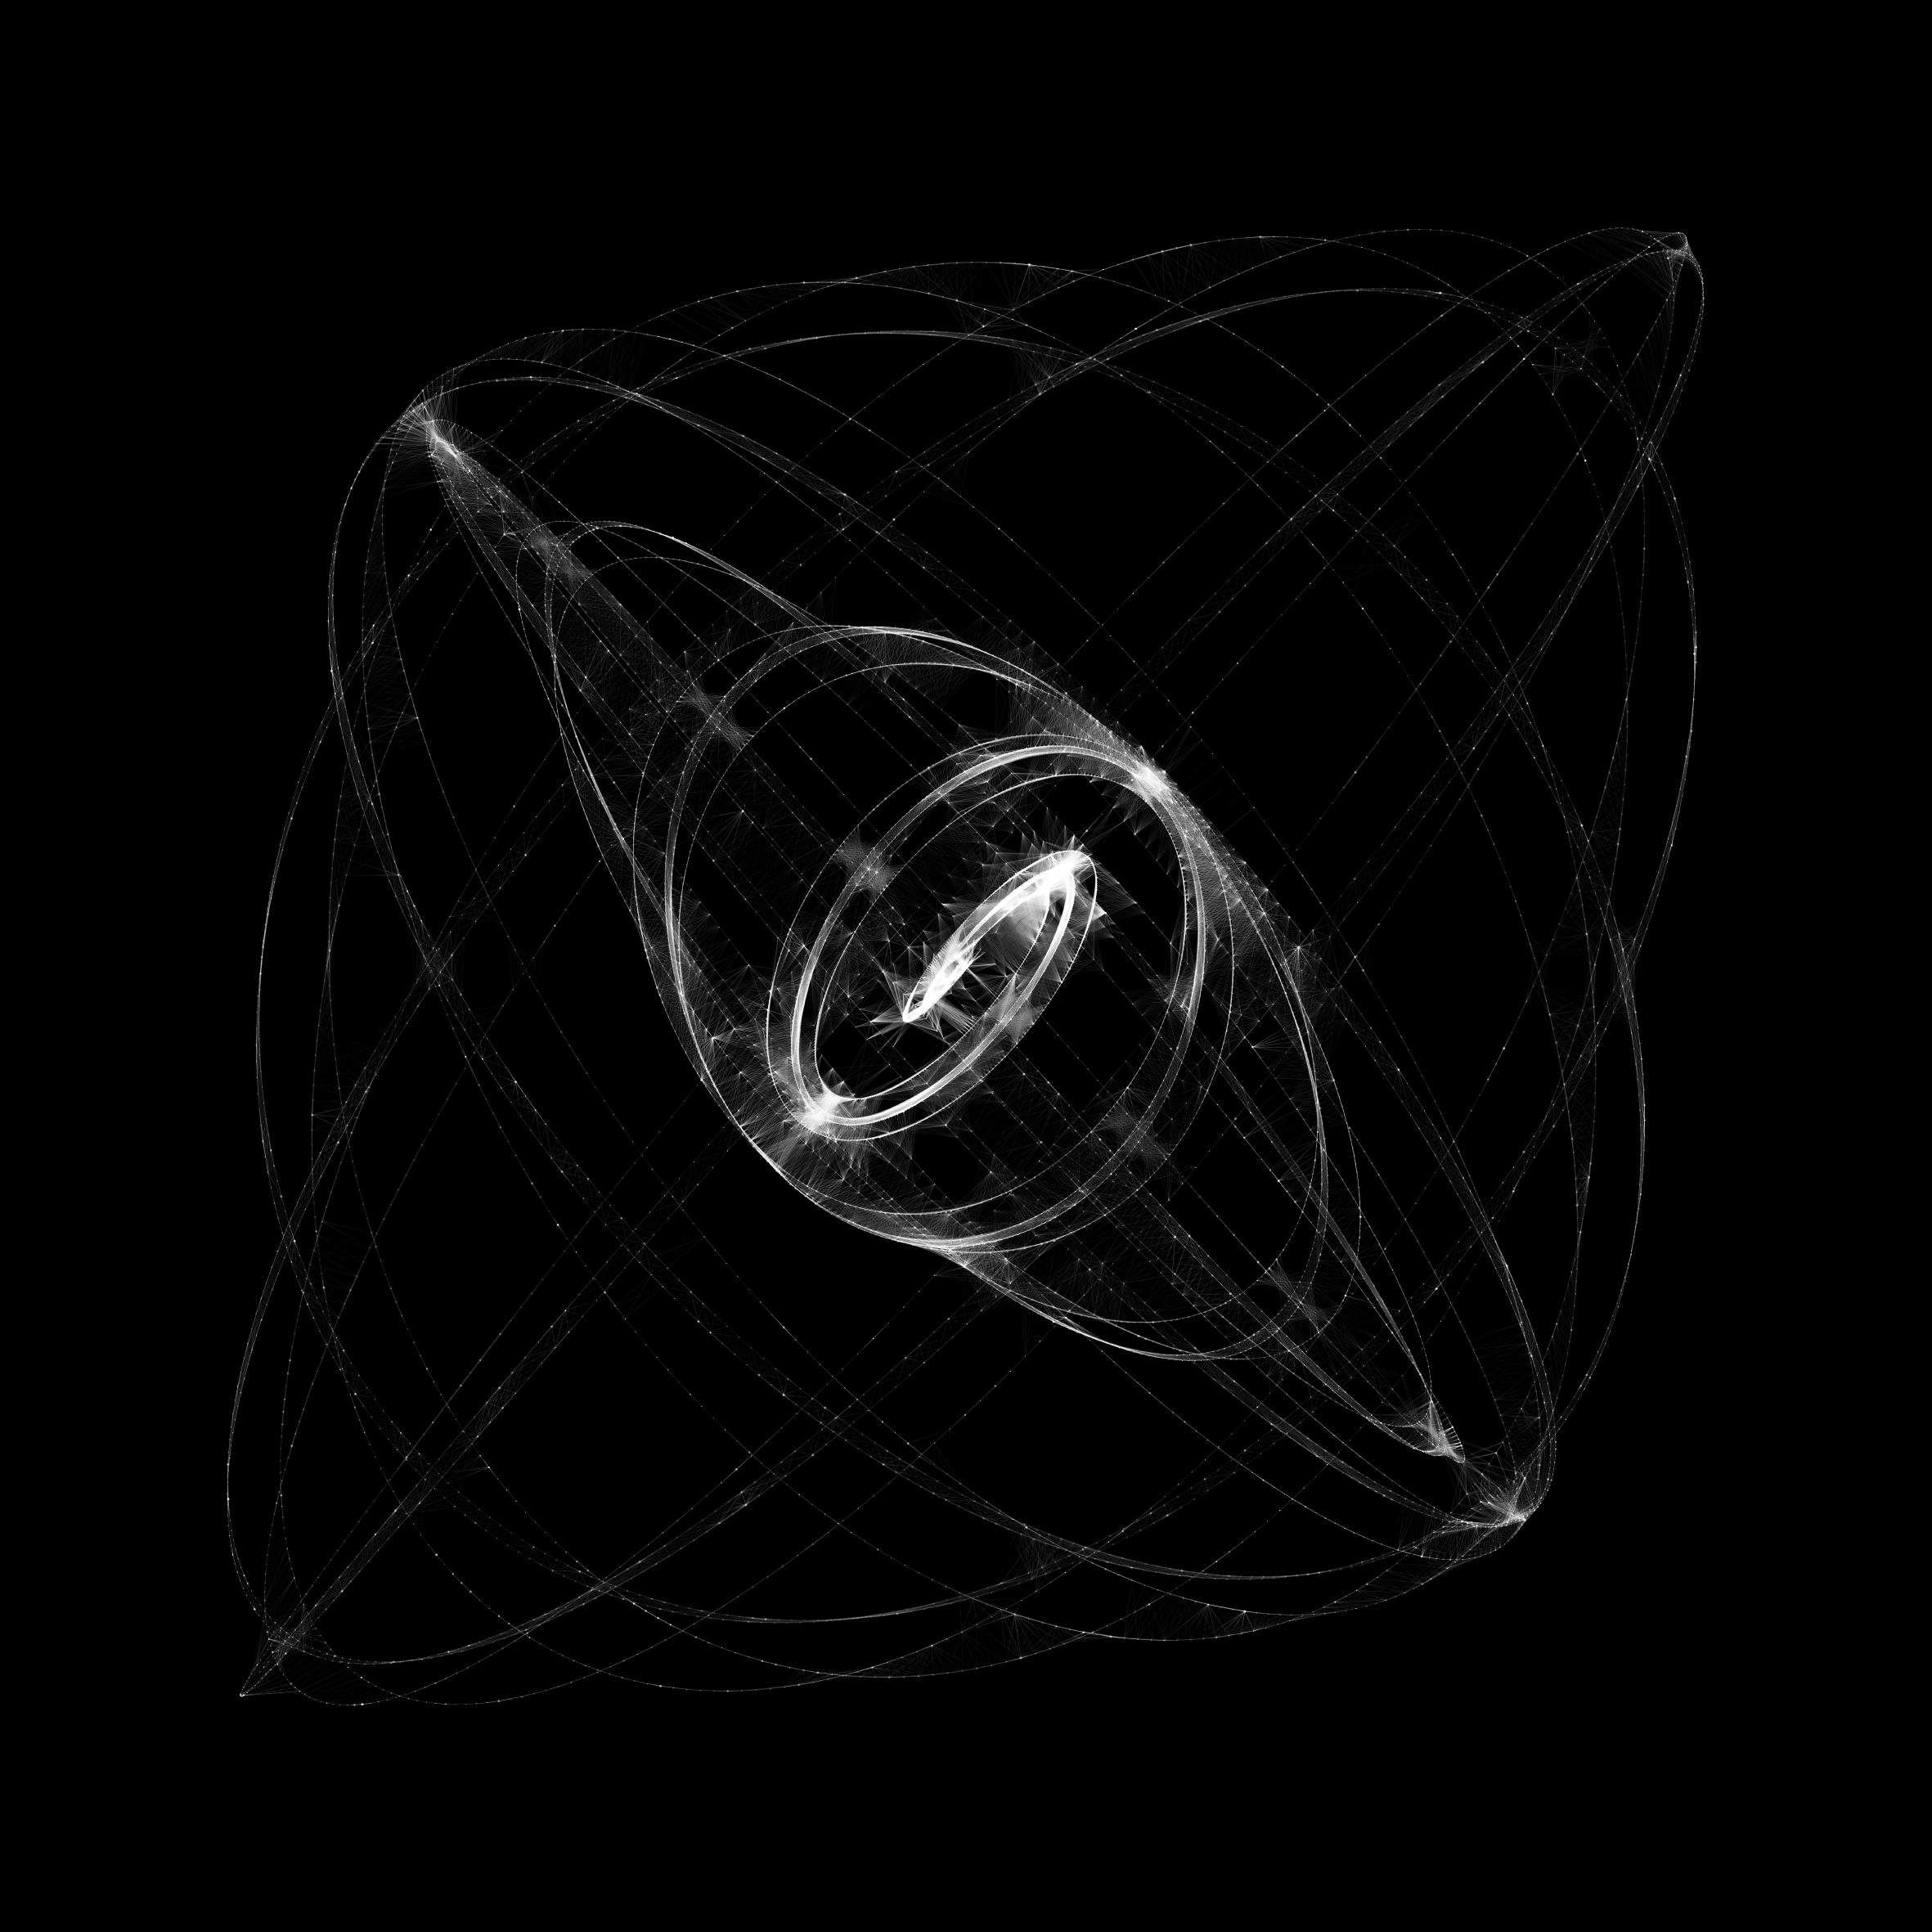
\includegraphics[width=0.6\textwidth]{Lissajous_Cashman}
\caption*{Segona major}
\end{figure}


\vfill

Author de la galeria: Ryan Cashman.
Text: Ryan Cashman


\section{Les Sèries Harmòniques}
Quan el Jules Antoine Lissajous va inventar el dispositiu que produeix les corbes amb el seu nom, va ser amb el propòsit d'estandarditzar els sons musicals. Al seu disseny original, dos diapasons es col·locaven de forma perpendicular, cadascun amb un mirall enganxat a un extrem. Llavors es feia incidir un feix de llum sobre el primer mirall, es reflectia cap al segon mirall i finalment a la pantalla. Si les freqüències dels diapasons tenien ràtios simples, cosa que els feia harmoniosos musicalment, les figures dibuixades amb la llum també ho eren visualment.

\begin{figure}[!h]
\centering
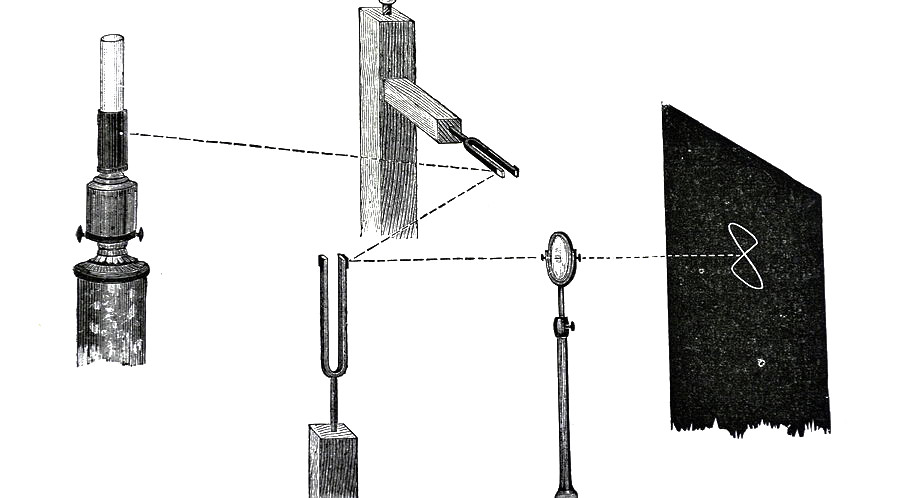
\includegraphics[width=0.6\textwidth]{Lissajous_apparatus}
\end{figure}

Les peces an aquestes sèries que van fer la Manuela Donoso i la Luisa Pereira recreen i estenen el dispositiu de Lissajous utilitzant tecnologia contemporània, portant-ho des del camp de la funcionalitat fins al de l'art interactiva. Els seus dispositius ens conviden a utilitzar les nostres veus per interactuar amb vibracions sonores de forma visual per desenvolupar un enteniment més profund i intuïtiu de la interacció entre soroll, consonància, dissonància i harmonia.

\subsection{Dispositiu \#1}
Micròfons, amplificadors, altaveus, miralls i làser.

Aquest dispositiu afegeix interactivitat a l'aparell original de Lissajous canviant els diapasons per altaveus i la font de llum per un punter làser. Cada altaveu es connecta a un micròfon i els dos miralls col·locats a les seves membranes vibren en direccions perpendiculars. Mentre els altaveus vibren amb les veus dels visitants, les figures projectades evolucionen: els sons percussius generen figures caòtiques, els intervals dissonants generen figures desordenades i els intervals consonants generen figures harmonioses. Si es xiula, les figures resultants són més agudes que si es canten les mateixes notes, fent visible la varietat i la riquesa del timbre a la música.


\subsection{Dispositiu \#2}
Micròfon, amplificador, convertidor analògic-digital, microcontrolador, sintetitzador i pantalla hologràfica.

Aquest dispositiu afegeix una tercera dimensió a les figures de Lissajous, permetent la visualització dels acords de triada. Les dues primeres notes les generen oscil·ladors i els visitants poden ajustar-ne la freqüència movent botons lliscants amunt o avall. La tercera vibració és la que els visitants triïn fer amb un micròfon: poden cantar diferents tons, parlar, xiuxiuejar o experimentar amb qualsevol so que els agradi. Aquest software personalitzat mostra aquestes tres vibracions en un espai tridimensional amb el temps: el primer sintetitzador determina la x, la veu la y i el segon sintetitzador la z de cada punt de la figura 3D resultant. Finalment, la figura es codifica per poder-la mostrar en una pantalla hologràfica, creant una estructura de llum que evoluciona constantment.

\subsection{Escultures de Triada}
Impressions 3D amb estereolitografia.

Les figures tridimensionals de Lissajous representen tres triades diferents: majors (amb ràtios de freqüència $4:5:6$), menors ($10:12:15$), i disminuïdes (aproximadament $20:24:29$). Observa que tant en el cas de les majors i menors, quan agafem parelles de freqüències aquestes tenen ràtios $4:5$, $5:6$, i $2:3$, però les figures de Lissajous (i els acords) no són el mateix. Pots utilitzar un focus per crear una ombra. El nombre de lòbuls a cada costat de la figura plana de Lissajous et dóna  les ràtios.

Aquestes figures es poden reproduir fent que el Dispositiu \#2 rebi tons amb aquestes ràtios, cantant i desplaçant els botons dels sintetitzadors.

\vfill

Autors de les sèries: Manuela Donoso i Luisa Pereira.
Producció (Dispositiu \#1): Manuela Donoso i Lukas Reck per IMAGINARY.
Programació (Dispositiu \#2): Luisa Pereira i Ricardo Dodds.

Patrocinat: Pantalla hologràfica 3D de The Looking Glass (\url{https://lookingglassfactory.com}).
Text: Manuela Donoso i Luisa Pereira.

Referències: \url{www.theharmonicseries.net}
